% NeurIPS Best Paper Style – clean, flat, minimal
\definecolor{NBlue}{HTML}{1A56A0}
\definecolor{NRed}{HTML}{C0392B}
\definecolor{NGreen}{HTML}{1A7A45}
\definecolor{NGold}{HTML}{B07D1A}
\definecolor{NSlate}{HTML}{4A5568}
\definecolor{NBlueFill}{HTML}{EBF2FB}
\definecolor{NRedFill}{HTML}{FBEAEA}
\definecolor{NGreenFill}{HTML}{EBF5EF}
\definecolor{NGoldFill}{HTML}{FDF6E3}
\definecolor{NSlateFill}{HTML}{F0F2F5}
\definecolor{NStroke}{HTML}{BBBDC2}

\begin{figure}[t!]
\centering
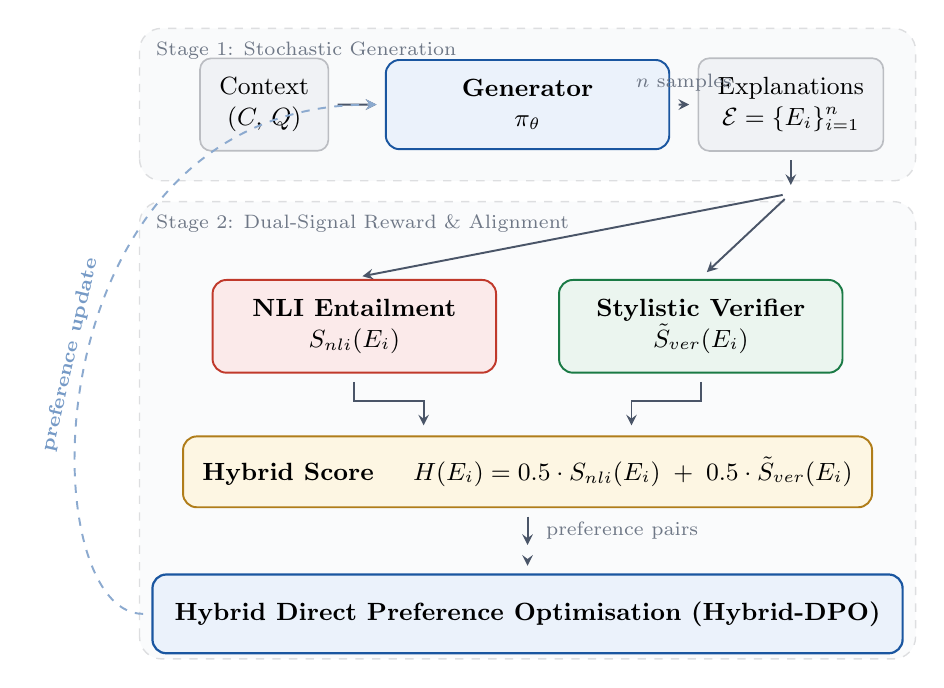
\begin{tikzpicture}[
    scale=0.88,
    >=stealth,
    % Core node styles
    iobox/.style={
        draw=NStroke, fill=NSlateFill,
        rounded corners=4pt, align=center,
        font=\small, inner sep=7pt, line width=0.6pt
    },
    modbox/.style={
        draw=#1, fill=#1Fill,
        rounded corners=5pt, align=center,
        font=\small\bfseries, inner sep=7pt,
        minimum height=1.0cm, minimum width=3.6cm,
        line width=0.7pt
    },
    gatebox/.style={
        draw=NGold, fill=NGoldFill,
        rounded corners=5pt, align=center,
        font=\small\bfseries, inner sep=7pt,
        minimum height=0.9cm, minimum width=8.0cm,
        line width=0.7pt
    },
    dpobox/.style={
        draw=NBlue, fill=NBlueFill,
        rounded corners=5pt, align=center,
        font=\small\bfseries, inner sep=8pt,
        minimum height=1.0cm, minimum width=9.0cm,
        line width=0.8pt
    },
    arr/.style={->, line width=0.7pt, color=NSlate, shorten >=3pt, shorten <=3pt},
    arrd/.style={->, line width=0.7pt, color=NBlue!50, dashed, shorten >=3pt, shorten <=3pt},
    steplabel/.style={font=\footnotesize\bfseries, color=NSlate},
    sublabel/.style={font=\scriptsize, color=NSlate!80}
]

%% -------------------------------------------------------
%% STAGE 1 background (subtle)
\draw[draw=NStroke!50, fill=NSlateFill!40, rounded corners=8pt, line width=0.5pt, dashed]
    (-5.6, 2.8) rectangle (5.6, 5.0);
\node[sublabel, anchor=north west] at (-5.5, 4.95) {Stage 1: Stochastic Generation};

%% STAGE 1: Input → Generator → Candidates
\node[iobox] (input) at (-3.8, 3.9) {Context\\$(C,\, Q)$};
\node[modbox=NBlue] (gen) at (0, 3.9) {Generator\\$\pi_{\theta}$};
\node[iobox] (cands) at (3.8, 3.9) {Explanations\\$\mathcal{E} = \{E_i\}_{i=1}^{n}$};

\draw[arr] (input) -- (gen);
\draw[arr] (gen) -- node[above, sublabel, yshift=1pt] {$n$ samples} (cands);

%% -------------------------------------------------------
%% STAGE 2 background
\draw[draw=NStroke!50, fill=NSlateFill!30, rounded corners=8pt, line width=0.5pt, dashed]
    (-5.6, -4.1) rectangle (5.6, 2.5);
\node[sublabel, anchor=north west] at (-5.5, 2.45) {Stage 2: Dual-Signal Reward \& Alignment};

%% Fan-out connector
\draw[arr] (cands.south) -- ++(0,-0.6) coordinate (fanout);
\draw[arr] (fanout) -- (-2.5, 1.4);
\draw[arr] (fanout) -- ( 2.5, 1.4);

%% REWARD COMPONENTS (two signals)
\node[modbox=NRed,   minimum width=3.6cm] (nli) at (-2.5, 0.7)
    {NLI Entailment\\$S_{\text{nli}}(E_i)$};
\node[modbox=NGreen, minimum width=3.6cm] (ver) at ( 2.5, 0.7)
    {Stylistic Verifier\\$\tilde{S}_{\text{ver}}(E_i)$};

%% Converge arrows
\draw[arr] (nli.south) -- ++(0,-0.4) -| (-1.5,-0.85);
\draw[arr] (ver.south) -- ++(0,-0.4) -| ( 1.5,-0.85);

%% HYBRID SCORE
\node[gatebox] (hybrid) at (0, -1.4)
    {Hybrid Score \quad
     $H(E_i) = 0.5 \cdot S_{\text{nli}}(E_i) \;+\; 0.5 \cdot \tilde{S}_{\text{ver}}(E_i)$};

%% DPO
\draw[arr] (hybrid.south) -- node[right, sublabel, xshift=3pt] {preference pairs} ++(0,-0.65) coordinate (mid);
\draw[arr] (mid) -- ++(0,-0.3);

\node[dpobox] (dpo) at (0, -3.45)
    {Hybrid Direct Preference Optimisation (Hybrid-DPO)};

%% FEEDBACK LOOP
\draw[arrd]
    (dpo.west)
    .. controls (-7.2, -3.45) and (-7.2, 3.9) ..
    (gen.west)
    node[midway, sloped, above, font=\scriptsize\bfseries, color=NBlue!60]
        {preference update};

\end{tikzpicture}
\caption{The \textbf{RLearner-LLM} framework. Stage~1 samples $n$ candidate explanations from the generator $\pi_\theta$. Stage~2 scores each candidate via two complementary signals---NLI entailment for logical correctness and a stylistic verifier for pedagogical quality---and combines them into a hybrid score. Preference pairs are formed from the scored pool and used to update $\pi_\theta$ via Hybrid-DPO.}
\label{fig:hybrid_dpo}
\end{figure}

\section{Methodology}
\label{sec:methodology}

\subsection{First-Principles Derivation of the Hybrid Reward}
\label{sec:first_principles}

\paragraph{The RLHF Objective and Its Core Tension.}
The canonical RLHF objective~\cite{ouyang2022training} is:
\begin{equation}
\max_{\pi_\theta}\; \mathbb{E}_{y \sim \pi_\theta(y|x)}\bigl[r(x,y)\bigr] - \beta\,\text{KL}\bigl(\pi_\theta \,\|\, \pi_\text{ref}\bigr)
\label{eq:rlhf}
\end{equation}
where $\pi_\text{ref}$ is the supervised fine-tuned reference policy and $\beta$ controls how much the learned policy is allowed to deviate from it.
DPO~\cite{rafailov2023direct} derives the closed-form optimal policy
$\pi^*(y|x) \propto \pi_\text{ref}(y|x)\cdot\exp(r(x,y)/\beta)$ and reformulates the objective as a direct binary cross-entropy loss on preference pairs, eliminating the need for an explicit reward model.

The KL term in Eq.~\ref{eq:rlhf} is the structural source of the \textbf{alignment tax}: it regularises the policy toward $\pi_\text{ref}$, which was trained via maximum-likelihood estimation (MLE) on human-written text. MLE by definition maximises fluency and surface coherence. Any reward signal that competes with this fluency prior---such as a pure NLI entailment objective---must overcome the KL gradient pulling the policy back toward verbose, fluent-but-logically-weak outputs.
This tension is not an implementation artefact; it is a structural consequence of Eq.~\ref{eq:rlhf} that persists regardless of the DPO variant used.

\paragraph{Why Single-Signal Optimization Fails.}
Two natural candidates for the reward signal $r(x,y)$ in educational explanation generation are NLI entailment probability and a stylistic quality verifier. However, each signal in isolation produces degenerate outcomes:

\begin{itemize}
    \item \textbf{NLI-only reward.} Maximising entailment probability $P_\text{NLI}(E \models A)$ alone causes the policy to converge toward short, answer-repeating snippets that satisfy the NLI scorer by simply restating the correct option---technically achieving high entailment while completely failing as an explanation. This is the alignment tax in its most extreme form: the model sacrifices all linguistic quality to maximise a single logical metric. Our ablation confirms this: NLI-only DPO on Qwen3-8B yields lower average NLI (0.172) than the additive Hybrid-DPO (0.198), because the degenerate short outputs do not generalise across diverse question types.
    \item \textbf{Verifier-only reward.} The Alpaca-7B verifier, trained on general fluency preferences, exhibits the same \textit{verbosity bias} as human annotators~\cite{zheng2024judging}: it systematically assigns high scores to longer, rhetorically polished responses. Verifier-only DPO therefore reinforces the SFT prior's tendency toward verbose, stylistically elaborate outputs, leaving the logical alignment gap unaddressed. This is precisely the failure mode documented in standard LLM-as-a-judge evaluation paradigms~\cite{wang2023large, pan2024evalbias}.
\end{itemize}

\paragraph{The Complementary Dual-Signal Hypothesis.}
Our key insight is that NLI entailment and verifier quality are \textit{complementary} rather than redundant: each captures a distinct dimension of explanation quality that the other misses.
NLI entailment $P_\text{NLI}(E \models A)$ measures whether the explanation logically implies the correct answer---a precise, verifiable property.
The verifier score $S_\text{ver}(E)$ measures holistic pedagogical quality, capturing properties such as clarity, coherent structure, and contextual appropriateness that an NLI classifier cannot detect.

Combining both signals ensures that a high-scoring explanation must be \textit{simultaneously} logically sound and linguistically natural: NLI corrects the verifier's verbosity blindspot, while the verifier prevents the degenerate short-form outputs that NLI-only optimization produces. We define the Hybrid reward as an equal-weight additive combination:
\begin{equation}
H(E) = 0.5 \cdot S_\text{NLI}(E) \;+\; 0.5 \cdot \tilde{S}_\text{ver}(E)
\label{eq:hybrid_reward}
\end{equation}
where $S_\text{NLI}(E) \in [0,1]$ is the DeBERTa-v3 NLI entailment probability and $\tilde{S}_\text{ver}(E) = (S_\text{ver}(E) - 1)/4$ normalises the Alpaca verifier's native $[1,5]$ scale to $[0,1]$, ensuring that both signals contribute equally to the composite score.

Equal weighting is a deliberate design choice: it prevents either signal from dominating the preference ordering. We also explore multiplicative reward composition and ACR-gated alternatives; these achieve comparable performance, confirming that the key innovation is the dual-signal design rather than the specific combination function (see ablation, Section~\ref{sec:ablation}).

\subsection{Preference Pair Construction}
\label{sec:pref_construction}

Given $n$ candidate explanations $\{E_i\}_{i=1}^n$ sampled from $\pi_\theta$ for a question-context pair $(C, Q)$, we score each candidate with $H(E_i)$ via Eq.~\ref{eq:hybrid_reward}. Pairs $(E_i, E_j)$ with $H(E_i) > H(E_j) + \Delta$ are retained as (chosen, rejected) pairs, where $\Delta \geq 0.03$ is a minimum score gap that ensures the signal-to-noise ratio of the preference label. This yields a dataset $\mathcal{D}_\text{pref} = \{(x_k, y_k^+, y_k^-)\}_{k=1}^K$ used to train Hybrid-DPO.

\subsection{Hybrid-DPO Training Objective}
\label{sec:hybrid_dpo}

The Hybrid-DPO objective follows the standard DPO formulation~\cite{rafailov2023direct} but is trained on $\mathcal{D}_\text{pref}$ constructed with the Hybrid reward (Eq.~\ref{eq:hybrid_reward}):
\begin{equation}
\mathcal{L}_\text{DPO}(\pi_\theta) = -\mathbb{E}_{(x,y^+,y^-)\sim\mathcal{D}_\text{pref}}\!\left[\log\sigma\!\left(\beta\!\left(\log\frac{\pi_\theta(y^+|x)}{\pi_\text{ref}(y^+|x)} - \log\frac{\pi_\theta(y^-|x)}{\pi_\text{ref}(y^-|x)}\right)\right)\right]
\label{eq:dpo_loss}
\end{equation}
Because every chosen example $y^+$ in $\mathcal{D}_\text{pref}$ is guaranteed to outscore its rejected counterpart on the dual-signal Hybrid score, the gradient of $\mathcal{L}_\text{DPO}$ consistently points toward higher joint logical-and-linguistic quality. This is the mechanism by which the dual-signal reward breaks the alignment tax that afflicts single-signal optimization.
